%16.10.2024, lecture 2

\section{Probabilistic approach}

Some intuition behing Shannon's entropy function.
Let $\alpha$ be a discrete random variable with values from the set $\{a_1, a_2, \ldots, a_k\}$ and probabilities $\{p_1, p_2, \ldots, p_k\}$, then \emph{Shannon Entropy} is:
\[
    H(\alpha) = \sum_i p_i \cdot (\text{information of } [\alpha = a_i]).
\]
In some sense, Shannons Entropy if the form of the expected value of the information we obtain from each outcome.

Some properties:
\begin{itemize}
    \item If $p_1 = \dots = p_k$, then $H(\alpha) = \log k$, so Shannon's entropy matches the Hartly's.
    \item If $p_1 = 1, p_2 = \dots = p_k = 0$, then $H(\alpha) = 0$.
\end{itemize}

\begin{figure}[H]
    \centering
    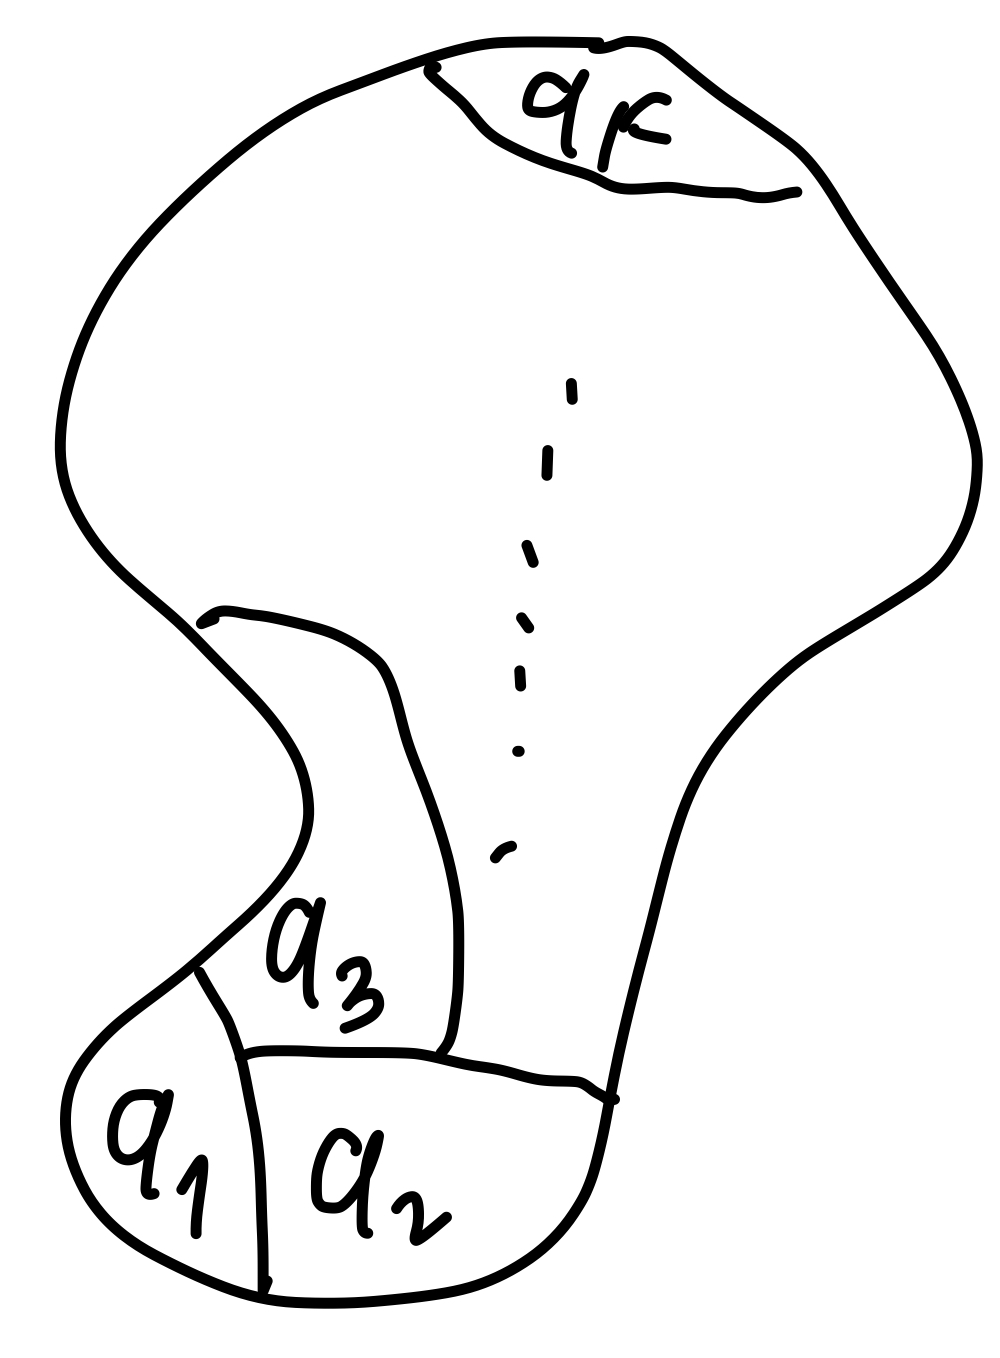
\includegraphics[width=0.15\textwidth]{figures/42D86984-D9AD-47FE-A062-3B83675568DA}
    \caption{Each area illustrates probability of an event.}
    \label{fig:42d86984-d9ad-47fe-a062-3b83675568da}
\end{figure}

How much information we get from an event that $\alpha = a_k$?
The initial measure of our set is $1$, but after getting that $\alpha = a_k$, we reduced the measure to $p_k$.
Hence, using Hartly's formula we get $-\log p_k$ information.
See \Cref{fig:42d86984-d9ad-47fe-a062-3b83675568da}.

\begin{definition}[1948]
    Shannon's entropy for a discrete random variable $\alpha$ is:
    \[
        H(\alpha) = \sum_i - p_i \log p_i.
    \]
\end{definition}
For continuity we define $0 \cdot \log 0 = 0$.

\begin{theorem}[Jensen's inequality]
    \label{thm:jensen}
    Let the function $f(x)$ be concave on some interval $\mathcal X$ and let the numbers $q_1, \ldots, q_n > 0$ be such that $\sum_i q_i = 1$.
    Then, for any $x_1, \ldots, x_n \in \mathcal X$ the inequality holds:
    \[
        \sum_{i = 1}^n q_i \cdot f(x_i) \leq f\left(\sum_{i = 1}^n q_i x_i\right).
    \]
    And it becomes an equality if and only if $q_i = 1$ and others $q_j = 0$.
\end{theorem}

\begin{lemma}
    The following holds:
    \begin{enumerate}
        \item $H(alpha) \geq 0$ for any $\alpha$.
        \item $H(\alpha) = 0 \iff $ the distribution of $\alpha$ is degenerate (constant).
        \item $H(\alpha) \leq \log k$ if and only if distribution of $\alpha$ is uniform.
    \end{enumerate}
\end{lemma}
\begin{proof}
    1, 2 ~-- trivial.
    3. Follows from the Jensen's inequality, see \Cref{thm:jensen}.
    \begin{align*}
        H(\alpha) - \log k = \sum_{i = 1}^k p_i \cdot \log \frac{1}{p_i} - \sum_{i = 1}^k p_i \log k = \sum_{i = 1}^k p_i \log \frac{1}{p_i k} \leq \log \sum_{i = 1}^k \frac{1}{k} = \log 1 = 0.
    \end{align*}
\end{proof}

\begin{definition}
    The entropy of the joint distribution of the pair of random variables $\alpha$, $\beta$ is  $H(\alpha, \beta)$.
\end{definition}
Basically, we create some random variable $\Delta = (\alpha, \beta)$.

\begin{lemma}
    \begin{enumerate}
        \item $H(\alpha, \beta) \leq H(\alpha) + H(\beta)$. And it is equality iff the random variables are independent.
        \item $ H(\alpha) \leq H(\alpha, \beta)$ and the equality iff $\beta =f(\alpha)$.
    \end{enumerate}
\end{lemma}
\begin{proof}
    Let $\alpha \in \{a_1, \ldots, a_k\}$ and $\beta \in \{b_1, \ldots, b_m\}$.
    And $p_{i, j} = \Pr[\alpha = a_i \land \beta = b_j]$.
    And let $p_{i,*} = \Pr[\alpha = a_i]$ and $p_{*, j} = \Pr[\beta = b_j]$.
    \begin{enumerate}
        \item
        \begin{align*}
            H(\alpha, \beta) - H(\alpha) - H(\beta) &= \sum_{i = 1}^{k} \sum_{j = 1}^{m} p_{i, j} \log \frac{1}{p_{i, j}} - \sum_{i = 1}^{k} p_{i,*} \log \frac{1}{p_{i,*}} - \sum_{j = 1}^m p_{*, j} \log \frac{1}{p_{*, j}} = \\
            &= \sum_{i = 1}^{k} \sum_{j = 1}^{m} p_{i, j} \log \frac{1}{p_{i, j}} - p_{i,j} \log \frac{1}{p_{i,*}} - p_{i, j} \log \frac{1}{p_{*, j}} = \\
            &= \sum_{i = 1}^k \sum_{j = 1}^m p_{i, j} \cdot \log \frac{p_{i,*} p_{j,*}}{p_{i, j}} \leq \\
            &\leq \log \sum_{i = 1}^k \sum_{j = 1}^m p_{i,*} p_{*,j} = \log 1 = 0.
        \end{align*}
        If $\alpha, \beta$ are independent, it is clear that we will have $0$ in the result.
        And vice versa, if we have $0$, it means that
        \[
            \sum_{i = 1}^k \sum_{j = 1}^m p_{i, j} \cdot \log \frac{p_{i,*} p_{j,*}}{p_{i, j}} = 0.
        \]
        Hence, $p_{i, *} p_{*, j} = p_{i, j}$.

        \item
        \begin{align*}
            H(\alpha) - H(\alpha, \beta) &= \sum_{i = 1}^k p_{i, *} \log \frac{1}{p_{i, *}} - \sum_{i = 1}^{k} \sum_{j = 1}^{m} p_i p_j \log \frac{1}{p_{i, j}} = \\
            & \sum_{i = 1}^k \sum_{j = 1}^m p_{i, j} \log \frac{1}{p_{i, *}} - \sum_{i = 1}^{k} \sum_{j = 1}^{m} p_{i, j} \log \frac{1}{p_{i, j}} = \\
            &= \sum_{i = 1}^k \sum_{j = 1}^m p_{i, j} \log \frac{p_{i, j}}{p_{i, *}} \leq \\
            &\leq \log \sum_{i = 1} \sum_{j = 1} p_{i, j} \underbrace{\frac{p_{i, j}}{p_{i, *}}}_{\leq 1} \leq \log 1 = 0.
        \end{align*}
        And now it is clear that it equals to $0$ iff $\beta = f(\alpha)$.
    \end{enumerate}
\end{proof}

\begin{definition}
    Given $\beta = \beta_i$, we say:
    \[
        H(\alpha \mid \beta = b_i) = \sum_{i} \Pr[\alpha = a_i \mid \beta = b_i] \cdot \log \frac{1}{\Pr[\alpha = a_i \mid \beta = b_i]}.
    \]
\end{definition}

\begin{definition}[Conditional entropy]
    \[
        H(\alpha \mid \beta) = \sum_j \Pr[\beta = b_j] \cdot H(\alpha \mid \beta = b_j).
    \]
\end{definition}
In other words,
\[
    H(\alpha \mid \beta) = \E_{\beta} [H(\alpha \mid \beta)].
\]

\begin{lemma}
    Following hols:
    \begin{enumerate}
        \item $H(\alpha \mid \beta) \geq 0$.
        \item  $H(\alpha \mid \beta) = 0$ iff  $\alpha$ is some $f(\beta)$.
        \item  $H(\alpha, \beta) = H(\beta) + H(\alpha \mid \beta) = H(\alpha) + H(\beta \mid \alpha)$.
    \end{enumerate}
\end{lemma}
\begin{proof}
    \begin{enumerate}
        \item It is a sum of non-negative values.
        \item Obviously.
        \item It is clear that $\Pr[\alpha = a_i \mid \beta = b_j] = \frac{p_{i, j}}{p_{*, j}}$, hence:
        \begin{align*}
            H(\alpha, \beta) &= H(\beta) + H(\alpha \mid \beta) &\iff \\
            \sum_{i, j} p_{i, j} \log \frac{1}{p_{i, j}} &= \sum_j p_{*, j} \log \frac{1}{p_{*, j}} + \sum_{i, j} p_{i, j} \log \frac{p_{*, j}}{p_{i, j}} &\iff \\
            \sum_{i, j} p_{i, j} \log \frac{1}{p_{i, j}} &= \sum_{i, j} p_{i, j} \left(\log \frac{1}{p_{*, j}} + \log \frac{p_{*, j}}{p_{i, j}}\right).
        \end{align*}
    \end{enumerate}
\end{proof}

\begin{corollary}
    For any $\alpha, \beta$ we have $H(\alpha \mid \beta) \leq H(\alpha)$ and the equation iff $\alpha, \beta$ are independent.
\end{corollary}
\begin{proof}
    We know that $H(\alpha, \beta) = H(\beta) + H(\alpha \mid \beta) \leq H(\alpha)$ and that $H(\alpha, \beta) \leq H(\alpha) + H(\beta)$.
    And the equation iff $H(\alpha, \beta) = H(\alpha) + H(\beta)$.
\end{proof}

\begin{definition}
    The information in $\alpha$ about $\beta$ is defined as:
    \[
        I(\alpha : \beta) = H(\beta) - H(\beta \mid \alpha).
    \]
\end{definition}

\begin{lemma}
    \begin{enumerate}
        \item $I(\alpha : \beta) \leq H(\alpha)$
        \item  $I(\alpha : \beta) \leq H(\beta)$
        \item  $I(\alpha : \alpha) = H(\alpha)$
        \item  $I(\alpha : \beta) = I(\beta : \alpha)$
        \item  $I(\alpha : \beta) = H(\alpha) + H(\beta) - H(\alpha, \beta)$.
    \end{enumerate}
\end{lemma}
\begin{proof}
    \begin{enumerate}
        \item Use point 4, then 2.
        \item Since $H(\beta \mid \alpha) \geq 0$.
        \item Since $H(\alpha \mid \alpha) = 0$.
        \item Follows from point 5.
        \item
        \begin{align*}
            I(\alpha : \beta) &= H(\alpha) + H(\beta) - H(\alpha, \beta) &\iff\\
            H(\alpha, \beta) &= H(\alpha) + H(\beta \mid \alpha).
        \end{align*}
    \end{enumerate}
\end{proof}

\begin{definition}
    The information in $\alpha$ about $\beta$ given $\gamma$ is defined as follows:
    \[I(\alpha : \beta \mid \gamma) = H(\beta \mid \gamma) - H(\beta \mid \alpha, \gamma)\]
\end{definition}
\begin{lemma}
    \begin{enumerate}
        \item  \[I(\alpha : \beta \mid \gamma) = \sum_l I(\alpha : \beta \mid \gamma = c_l) \cdot \Pr[\gamma = c_l]\] (expectation of $E_\gamma I(\alpha : \beta \mid \gamma)$)
        \item $I(\alpha : \beta \mid \gamma) = H(\alpha \mid \gamma) + H(\beta \mid \gamma) - H(\alpha, \beta \mid \gamma)$
        \item  $I(\alpha : \beta \mid \gamma) = H(\alpha, \gamma) + H(\beta, \gamma) - H(\alpha, \beta, \gamma) - H(\gamma)$

    \end{enumerate}
\end{lemma}

\begin{lemma}
    The following holds:
    \begin{enumerate}
        \item $I((a, b) : \gamma) = I(\alpha : \gamma) + I(\beta : \gamma \mid \alpha)$
        \item  $I((\alpha, \beta) : \gamma \mid \delta) = I(\alpha : \gamma \mid \delta) + I(\beta : \gamma \mid \alpha, \delta)$
    \end{enumerate}
\end{lemma}

We can use Euler's circles to illustrate entropies.
See \Cref{fig:ae3e659e-8b57-4c03-b616-54b5facac858,fig:c3ccbafa-9451-4d04-bbf1-b50dc41cf6fd}

\begin{figure}[H]
    \centering
    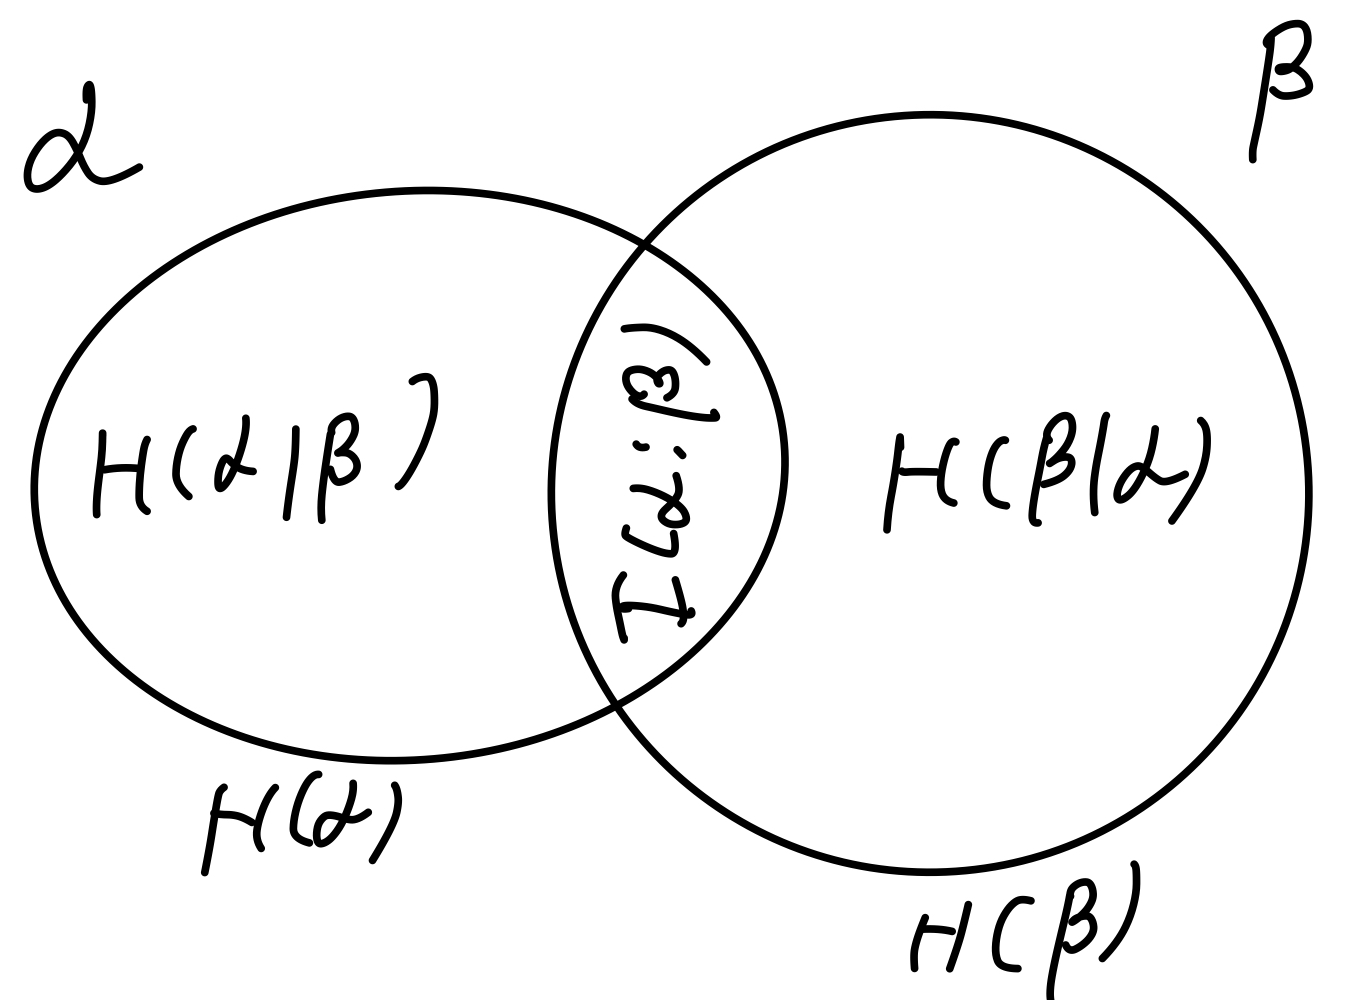
\includegraphics[width=0.3\textwidth]{figures/AE3E659E-8B57-4C03-B616-54B5FACAC858}
    \caption{Euler's circles for two variables.}
    \label{fig:ae3e659e-8b57-4c03-b616-54b5facac858}
\end{figure}

\begin{figure}[H]
    \centering
    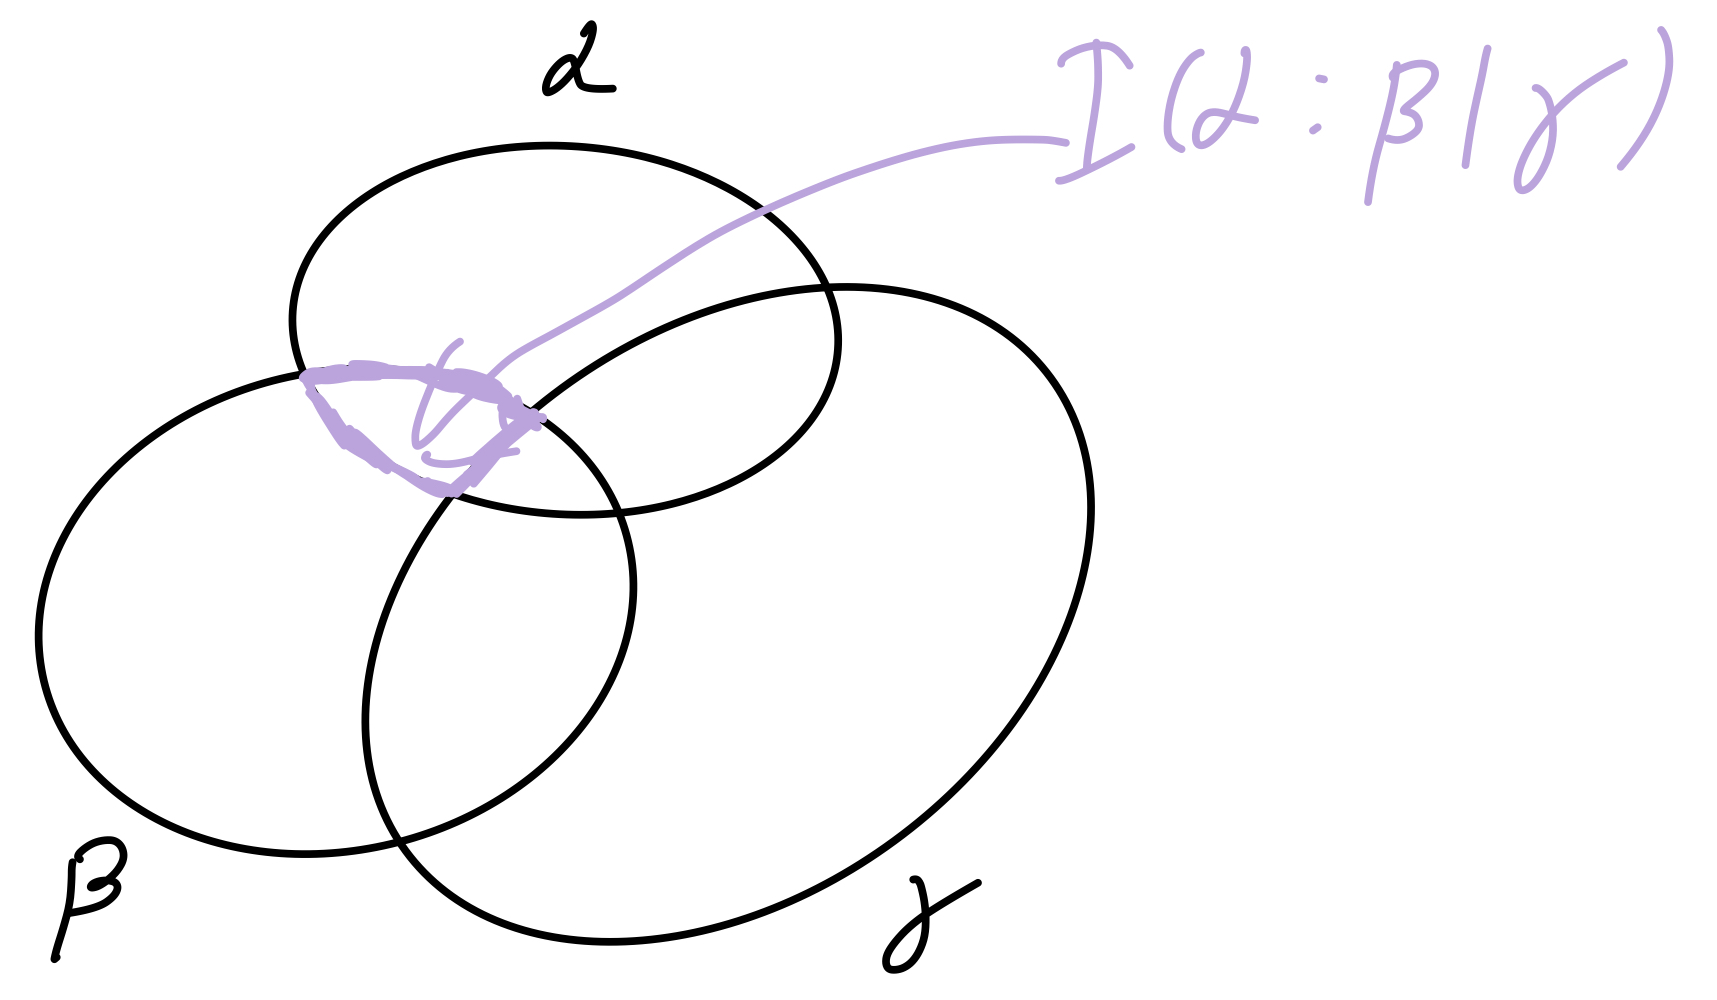
\includegraphics[width=0.3\textwidth]{figures/C3CCBAFA-9451-4D04-BBF1-B50DC41CF6FD}
    \caption{Euler's circles three two variables.}
    \label{fig:c3ccbafa-9451-4d04-bbf1-b50dc41cf6fd}
\end{figure}

Now, the lemmas above are clear.

\begin{definition}
    \[
        I(\alpha : \beta : \gamma) = I(\alpha : \beta) - I(\alpha : \beta \mid \gamma).
    \]
\end{definition}
\begin{lemma}
    $I(\alpha : \beta : \gamma)$ can be negative.
\end{lemma}
\begin{proof}
    Suppose $\alpha, \beta, \gamma \in \{0, 1\}$.
    And let $\gamma = \alpha \oplus \beta$ and $\alpha, \beta$ are uniform.
    Hence, $I(\alpha \colon \beta) = 0$.
    And  $I(\alpha : \beta \mid \gamma) = H(\beta \mid \gamma) - H(\beta \mid \alpha, \gamma) = 1$.
    Hence,  $I(\alpha : \beta : \gamma) = -1$.
    See \Cref{fig:33e03ecb-3aaa-4ef8-98af-42039ab45307} for more details.
    \begin{figure}[H]
        \centering
        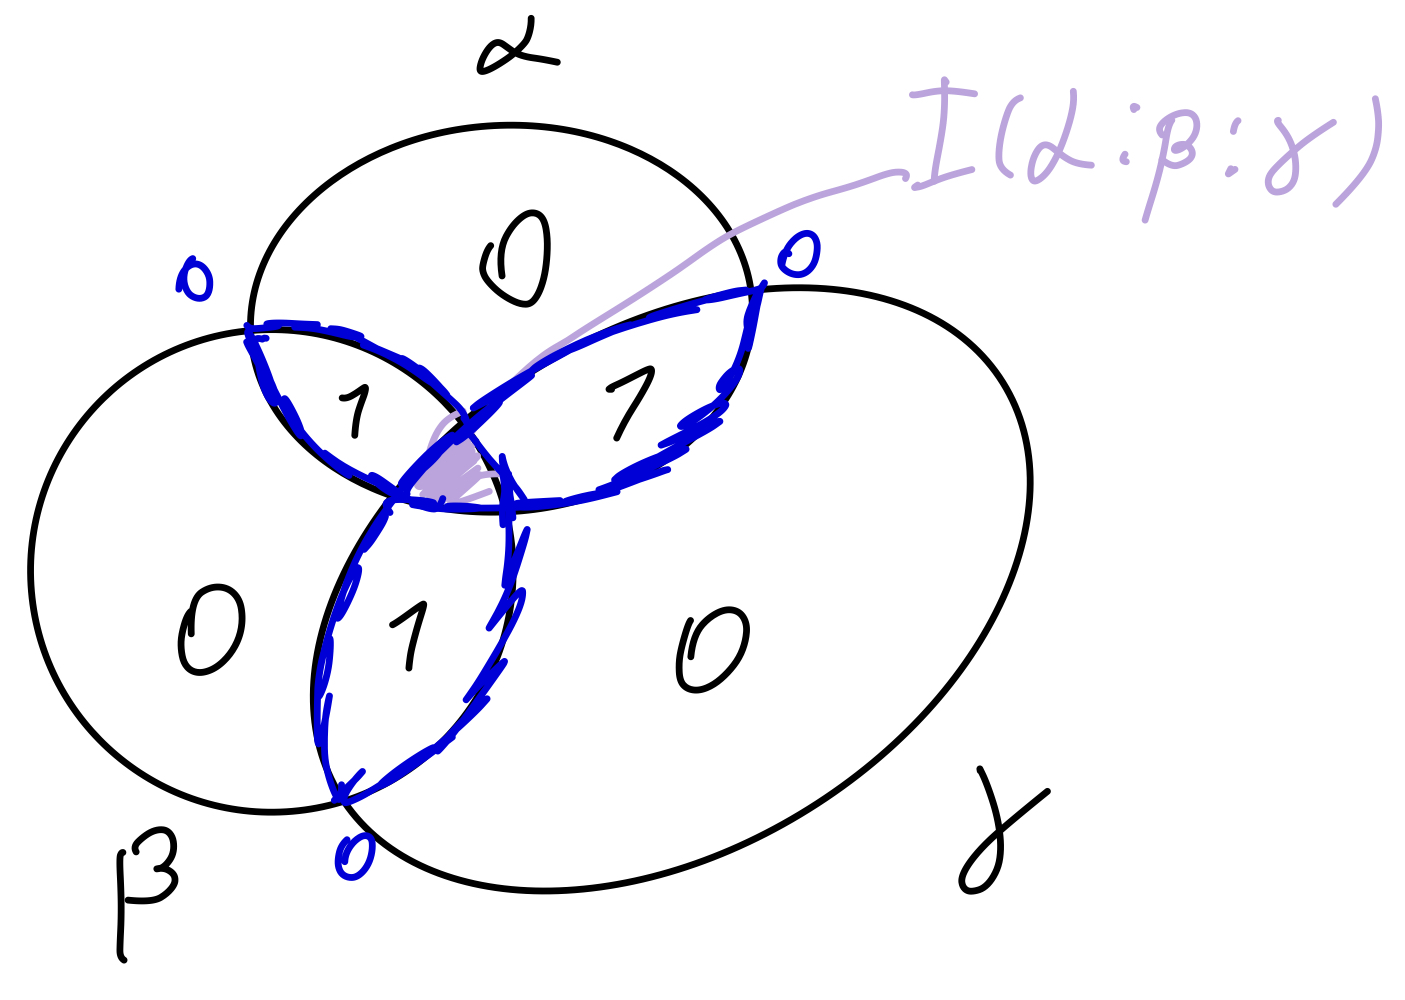
\includegraphics[width=0.4\textwidth]{figures/33E03ECB-3AAA-4EF8-98AF-42039AB45307}
        \caption{Counter example.}
        \label{fig:33e03ecb-3aaa-4ef8-98af-42039ab45307}
    \end{figure}

\end{proof}



\begin{exercise}
    Prove that Shannon entropy is not less than the minimum entropy, defined as $H_{\min} = \min (- \log p_i)$.
\end{exercise}
\begin{proof}
    \[
        H = -\sum_i p_i \log p_i \geq H_{\min}. \qedhere
    \]
\end{proof}

\begin{exercise}
    Let probabilities of random variable $\alpha$ be $\frac{1}{2}, \frac{1}{4}, \ldots, \frac{1}{2^{n - 1}}, \frac{1}{2^{n}}, \frac{1}{2^{n}}$.
    What does its entropy approach as $n \to \infty$?
    And the same question for variable $\beta$  with probabilities $\frac{1}{3}, \frac{1}{3}, \frac{1}{9}, \frac{1}{9}, \dots, \frac{1}{3^{n - 1}}, \frac{1}{3^{n - 1}}, \frac{1}{3^{n}}, \frac{1}{3^{n}}, \frac{1}{3^{n}}$.
\end{exercise}
\begin{proof}
    It is clear that $-\log \frac{1}{2^{k}} = k$, hence $\frac{1}{2^{k}} \cdot \log 2^{k} = \frac{k}{2^{k}}$, thus
    \begin{align*}
        H(\alpha) = \sum_k \frac{k}{2^{k}} = 2
    \end{align*}

%    Now, since $\log_3 (x) = \log_2(x) \cdot \log_3(2)$, hence $H(\beta) = 4 \cdot \log_3(2)$.
%    \todo{correct}
\end{proof}
